\documentclass[12pt]{article}

\usepackage[utf8x]{inputenc} % Включаем поддержку UTF8  
\usepackage[russian]{babel}  % Включаем пакет для поддержки русского языка  
\usepackage{hyperref}        % Для гиперссылок

% Математика
\usepackage{amsmath,amsfonts,amssymb,amsthm,mathtools} % AMS
\usepackage{icomma}
\usepackage{mathrsfs}

\usepackage{xcolor}

% Прога
\usepackage{etoolbox}
\usepackage{listings}

\definecolor{codegreen}{rgb}{0,0.6,0}
\definecolor{codegray}{rgb}{0.5,0.5,0.5}
\definecolor{codepurple}{rgb}{0.58,0,0.82}
\definecolor{backcolour}{rgb}{0.95,0.95,0.92}

\lstdefinestyle{mystyle}{
	backgroundcolor=\color{backcolour},   
	commentstyle=\color{codegreen},
	keywordstyle=\color{magenta},
	numberstyle=\tiny\color{codegray},
	stringstyle=\color{codepurple},
	basicstyle=\ttfamily\footnotesize,
	breakatwhitespace=false,         
	breaklines=true,                 
	captionpos=b,                    
	keepspaces=true,                 
	numbers=left,                    
	numbersep=5pt,                  
	showspaces=false,                
	showstringspaces=false,
	showtabs=false,                  
	tabsize=2
}

\lstset{style=mystyle}

% Цвета
\usepackage{xcolor}

% Картинки
\usepackage{graphicx}
\graphicspath{ {./images/} }

\usepackage{tikzsymbols}

% Работа с таблицами
\usepackage{array,tabularx,tabulary,booktabs} % Дополнительная работа с таблицами
\usepackage{longtable}  % Длинные таблицы
\usepackage{multirow} % Слияние строк в таблице

% Нумерованные списки
\usepackage[shortlabels]{enumitem} % Разные лейблы

% Текст
\usepackage[normalem]{ulem}  % для зачеркивания текста

\newtheorem{property}{Свойство}
\newtheorem{consequence}{Следствие}[property]

\DeclarePairedDelimiter\abs{\lvert}{\rvert}%
\DeclarePairedDelimiter\norm{\lVert}{\rVert}%

% Swap the definition of \abs* and \norm*, so that \abs
% and \norm resizes the size of the brackets, and the 
% starred version does not.
\makeatletter
\let\oldabs\abs
\def\abs{\@ifstar{\oldabs}{\oldabs*}}
%
\let\oldnorm\norm
\def\norm{\@ifstar{\oldnorm}{\oldnorm*}}
\makeatother

\begin{document}
	
	\thispagestyle{empty}
	\begin{center}
		\textbf{ПРАВИТЕЛЬСТВО РОССИЙСКОЙ ФЕДЕРАЦИИ}
		
		\vspace{5ex}
		
		\textbf{Федеральное государственное автономное образовательное учреждение \\ высшего образования \\ <<Национальный исследовательский университет \\ <<Высшая школа экономики>>}
	\end{center}
	\vspace{5ex}
	
	\begin{center}
		Московский институт электроники и математики им. А.Н. Тихонова  
		
		\vspace{5ex}
		
		Департамент прикладной математики
		
		\vspace{10ex}
		\textbf{Отчёт \\ по лабораторной работе №2 \\ по курсу <<Алгоритмизация и программирование>> \\ Задание № 13}
		\vspace{7ex}
		
	\end{center}
	
	\begin{center} 
		\begin{tabular}{| p{0.3\linewidth}| p{0.3\linewidth}| p{0.3\linewidth}|}
			\hline	
			ФИО студента & Номер группы & Дата \\  \hline
			& & \\  
			Кейер Александр \newline Петрович & БПМ-231 & 14.10.2023\\  
			& & \\  \hline		
		\end{tabular}
	\end{center}
	
	\begin{center}
		\vspace{3ex}
		
		\vfill
		
		\normalsize
		
		\textbf{Москва, 2023}
	\end{center}
	
	\newpage
	
	%---------------------------------------------------------------------------------
	
	\section*{Задание (вариант № 13)}
	
	Даны числа x и y. Определить, принадлежит ли точка с координатами (x, y) заштрихованной области включая границы.
	\vspace{5px}
	\newline
	Оформить первое решение в виде вложенных условных операторов с простыми условиями.
	\vspace{5px}
	\newline
	Второе решение должно содержать один условный оператор со сложным логическим условием.
	\vspace{5px}
	\newline
	Третье решение должно быть оформлено в виде отдельной функции, вызываемой из основной программы. Функция не содержит условного оператора, а только логическое выражение.
		
	$$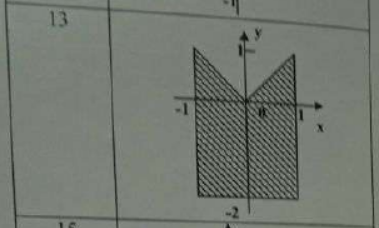
\includegraphics{task}$$
	
	\newpage
	
	\section*{Решение}
	
	\begin{lstlisting}[language=C]
	#include <stdio.h> // Input/output library.
	#include <math.h> // Math library.
	
	// Function checking dot containing.
	int isContainDot(double x, double y) {
		return (x >= 0 && x <= 1 && y >= -2 && y <= x) || (x < 0 && x >= -1 && y >= -2 && y <= -x); 
	}
	
	int main() {
		// Greeting.
		printf("Lab #2 made by Alexander Keyer from BAM231 group.\n\n");
		
		double x, y;
		
		// Friendly input interface.
		printf("Please, enter two float numbers \"x\" and \"y\" separated by a space: ");
		scanf("%lf %lf", &x, &y);
		
		printf("Solution 1: ");
		
		// First solution. Checking dot position
		if (x >= 0) {
			// First x half check.
			if (x <= 1) {
				// Frist y half check.
				if (y >= -2) {
					// First diagonal check.
					if (y <= x) {
						printf("Is figure contain dot: true");
					} else {
						printf("Is figure contain dot: false");
					}
				} else {
					printf("Is figure contain dot: false");
				}
			} else {
				printf("Is figure contain dot: false");
			}
		} else {
			// Second x half check.
			if (x >= -1) {
				// Second y half check.
				if (y >= -2) {
					// Second diagonal check.
					if (y <= -x) {
						printf("Is figure contain dot: true"); 
					} else {
						printf("Is figure contain dot: false");
					}
				} else {
					printf("Is figure contain dot: false");
				}
			} else {
				printf("Is figure contain dot: false");
			}
		}
		
		printf("\nSolution 2: ");
		
		// Second solution. Checking dot position
		if ((x >= 0 && x <= 1 && y >= -2 && y <= x) || (x < 0 && x >= -1 && y >= -2 && y <= -x)) {
			printf("Is figure contain dot: true");
		} else {
			printf("Is figure contain dot: false");
		}
		
		printf("\nSolution 3: ");
		
		// Third solution. Checking dot position
		if (isContainDot(x, y)) {
			printf("Is figure contain dot: true");
		} else {
			printf("Is figure contain dot: false");
		}
		
		return 0;
	}
	\end{lstlisting}
	
	\newpage
	
	\section*{Тесты}
	
	\subsection*{Тест № 1}
	\textit{Ввод:} 1 1 \newline
	\textit{Вывод:}
	\vspace{6px}
	\newline
	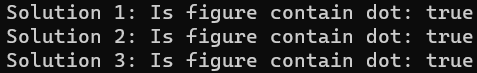
\includegraphics{test_1}
	\vspace{3px}
	\newline
	Программа сработала корректно.
	
	\subsection*{Тест № 2}
	\textit{Ввод:} 0.1234567 0.1234568 \newline
	\textit{Вывод:}
	\vspace{6px}
	\newline
	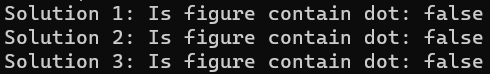
\includegraphics{test_2}
	\vspace{3px}
	\newline
	Программа сработала корректно.
	
	\subsection*{Тест № 3}
	\textit{Ввод:} -1 -1.987654321 \newline
	\textit{Вывод:}
	\vspace{6px}
	\newline
	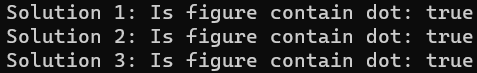
\includegraphics{test_3}
	\vspace{3px}
	\newline
	Программа сработала корректно.
	
	
	
\end{document}
